\documentclass[fontsize=17pt]{article}
% !TeX spellcheck = en_GB 

% Used in desctiption 
\usepackage{calc}
\usepackage{enumitem}
%

\renewcommand{\baselinestretch}{1.5}
\usepackage{array,tabularx}
\usepackage{arxiv_covid}
\usepackage{chngcntr}
\usepackage{amsmath}
\usepackage{fontawesome}
\usepackage[utf8]{inputenc} % allow utf-8 input
\usepackage[T1]{fontenc}    % use 8-bit T1 fonts
\usepackage{hyperref}       % hyperlinks
\usepackage{url}            % simple URL typ
\usepackage{booktabs}       % professional-quality tables
\usepackage{amsfonts}       % blackboard math symbols
\usepackage{nicefrac}       % compact symbols for 1/2, etc.
\usepackage{microtype}      % microtypography
\usepackage{lipsum}
\usepackage[utf8]{inputenc} % Required for inputting international characters
\usepackage[T1]{fontenc} % Output font encoding for international characters
\usepackage{pgfplots}
\usepackage{graphicx}
\usepackage{fancyhdr}
\usepackage{mathpazo} % Palatino font
\usepackage{mathrsfs}
\hypersetup{%
	pdfborder = {0 0 0}
}


\usepackage[T1]{fontenc}
\usepackage[utf8]{inputenc}
\usepackage{charter}
\usepackage{environ}

%---------------------
\usepackage{tikz}
\usetikzlibrary{fadings,positioning,calc,shadows,calc,matrix,shapes.geometric, arrows,positioning,chains}

\usetikzlibrary{arrows.meta} 

\usepackage{nameref}
\definecolor{lightgray}{gray}{0.9}
%\addbibresource{sample.bib} %Import the bibliography file
\usepackage{adjustbox}
\usepackage{pdflscape}
\providecommand{\abs}[1]{\lvert#1\rvert} %used for absolute value vertical bars 
\usepackage{changepage}% http://ctan.org/pkg/changepage
\usepackage{lmodern}
%---------------------

\fancyhf{}
\pagestyle{fancy}
%\renewcommand{\headrulewidth}{0pt}
\fancyheadoffset{2pt}
%\cfoot{\thepage}

\fancyhead[RE,LO]{\raisebox{1.3\height}\leftmark}
%\fancyhead[RO,LE]{\raisebox{1.3\height}\rightmark}
\fancyhead[LE,RO]{\raisebox{1.3\height}{Coronavirus (COVD-19, SARS-CoV-2)}}

\fancyfoot[LE,CO]{\raisebox{-1\height} {Page \thepage}}
\graphicspath{{_images_tables_figures/}}
\title{Mathematical Modelling of Infectious Diseases\\
\emph{Coronavirus (COVD-19, SARS-CoV-2)} }

\author{
	Ali~Al-Hayki\thanks{Use footnote for providing further
		information about author (webpage, alternative
		address)---\emph{not} for acknowledging funding agencies.} \\
	\faEnvelopeO \quad \href{mailto:ali.hayki@gmail.com}{\nolinkurl{
			ali.hayki@gmail.com} }\\
	\faGithub \quad \texttt{\href{https://github.com/hayki}{alihayki}}\\
	\faLinkedin \quad \texttt{\href{https://linedin.com/in/ali-al-hayki-17baa180/}{ali-al-hayki}}\\
}
\date{23/03/2020}

%Colors
%--------------------
\definecolor{aquamarine}{rgb}{0.5, 1.0, 0.83}
\definecolor{airforceblue}{rgb}{0.36, 0.54, 0.66}
\definecolor{aqua}{rgb}{0.0, 1.0, 1.0}
\definecolor{babyblue}{rgb}{0.54, 0.81, 0.94}
\definecolor{atomictangerine}{rgb}{1.0, 0.6, 0.4}
\definecolor{bluegray}{rgb}{0.4, 0.6, 0.8}
%--------------------

%Timeline
%-----------------------------

%-----------------------------

\begin{document}
	
\maketitle



\begin{figure}
	\begin{center}
	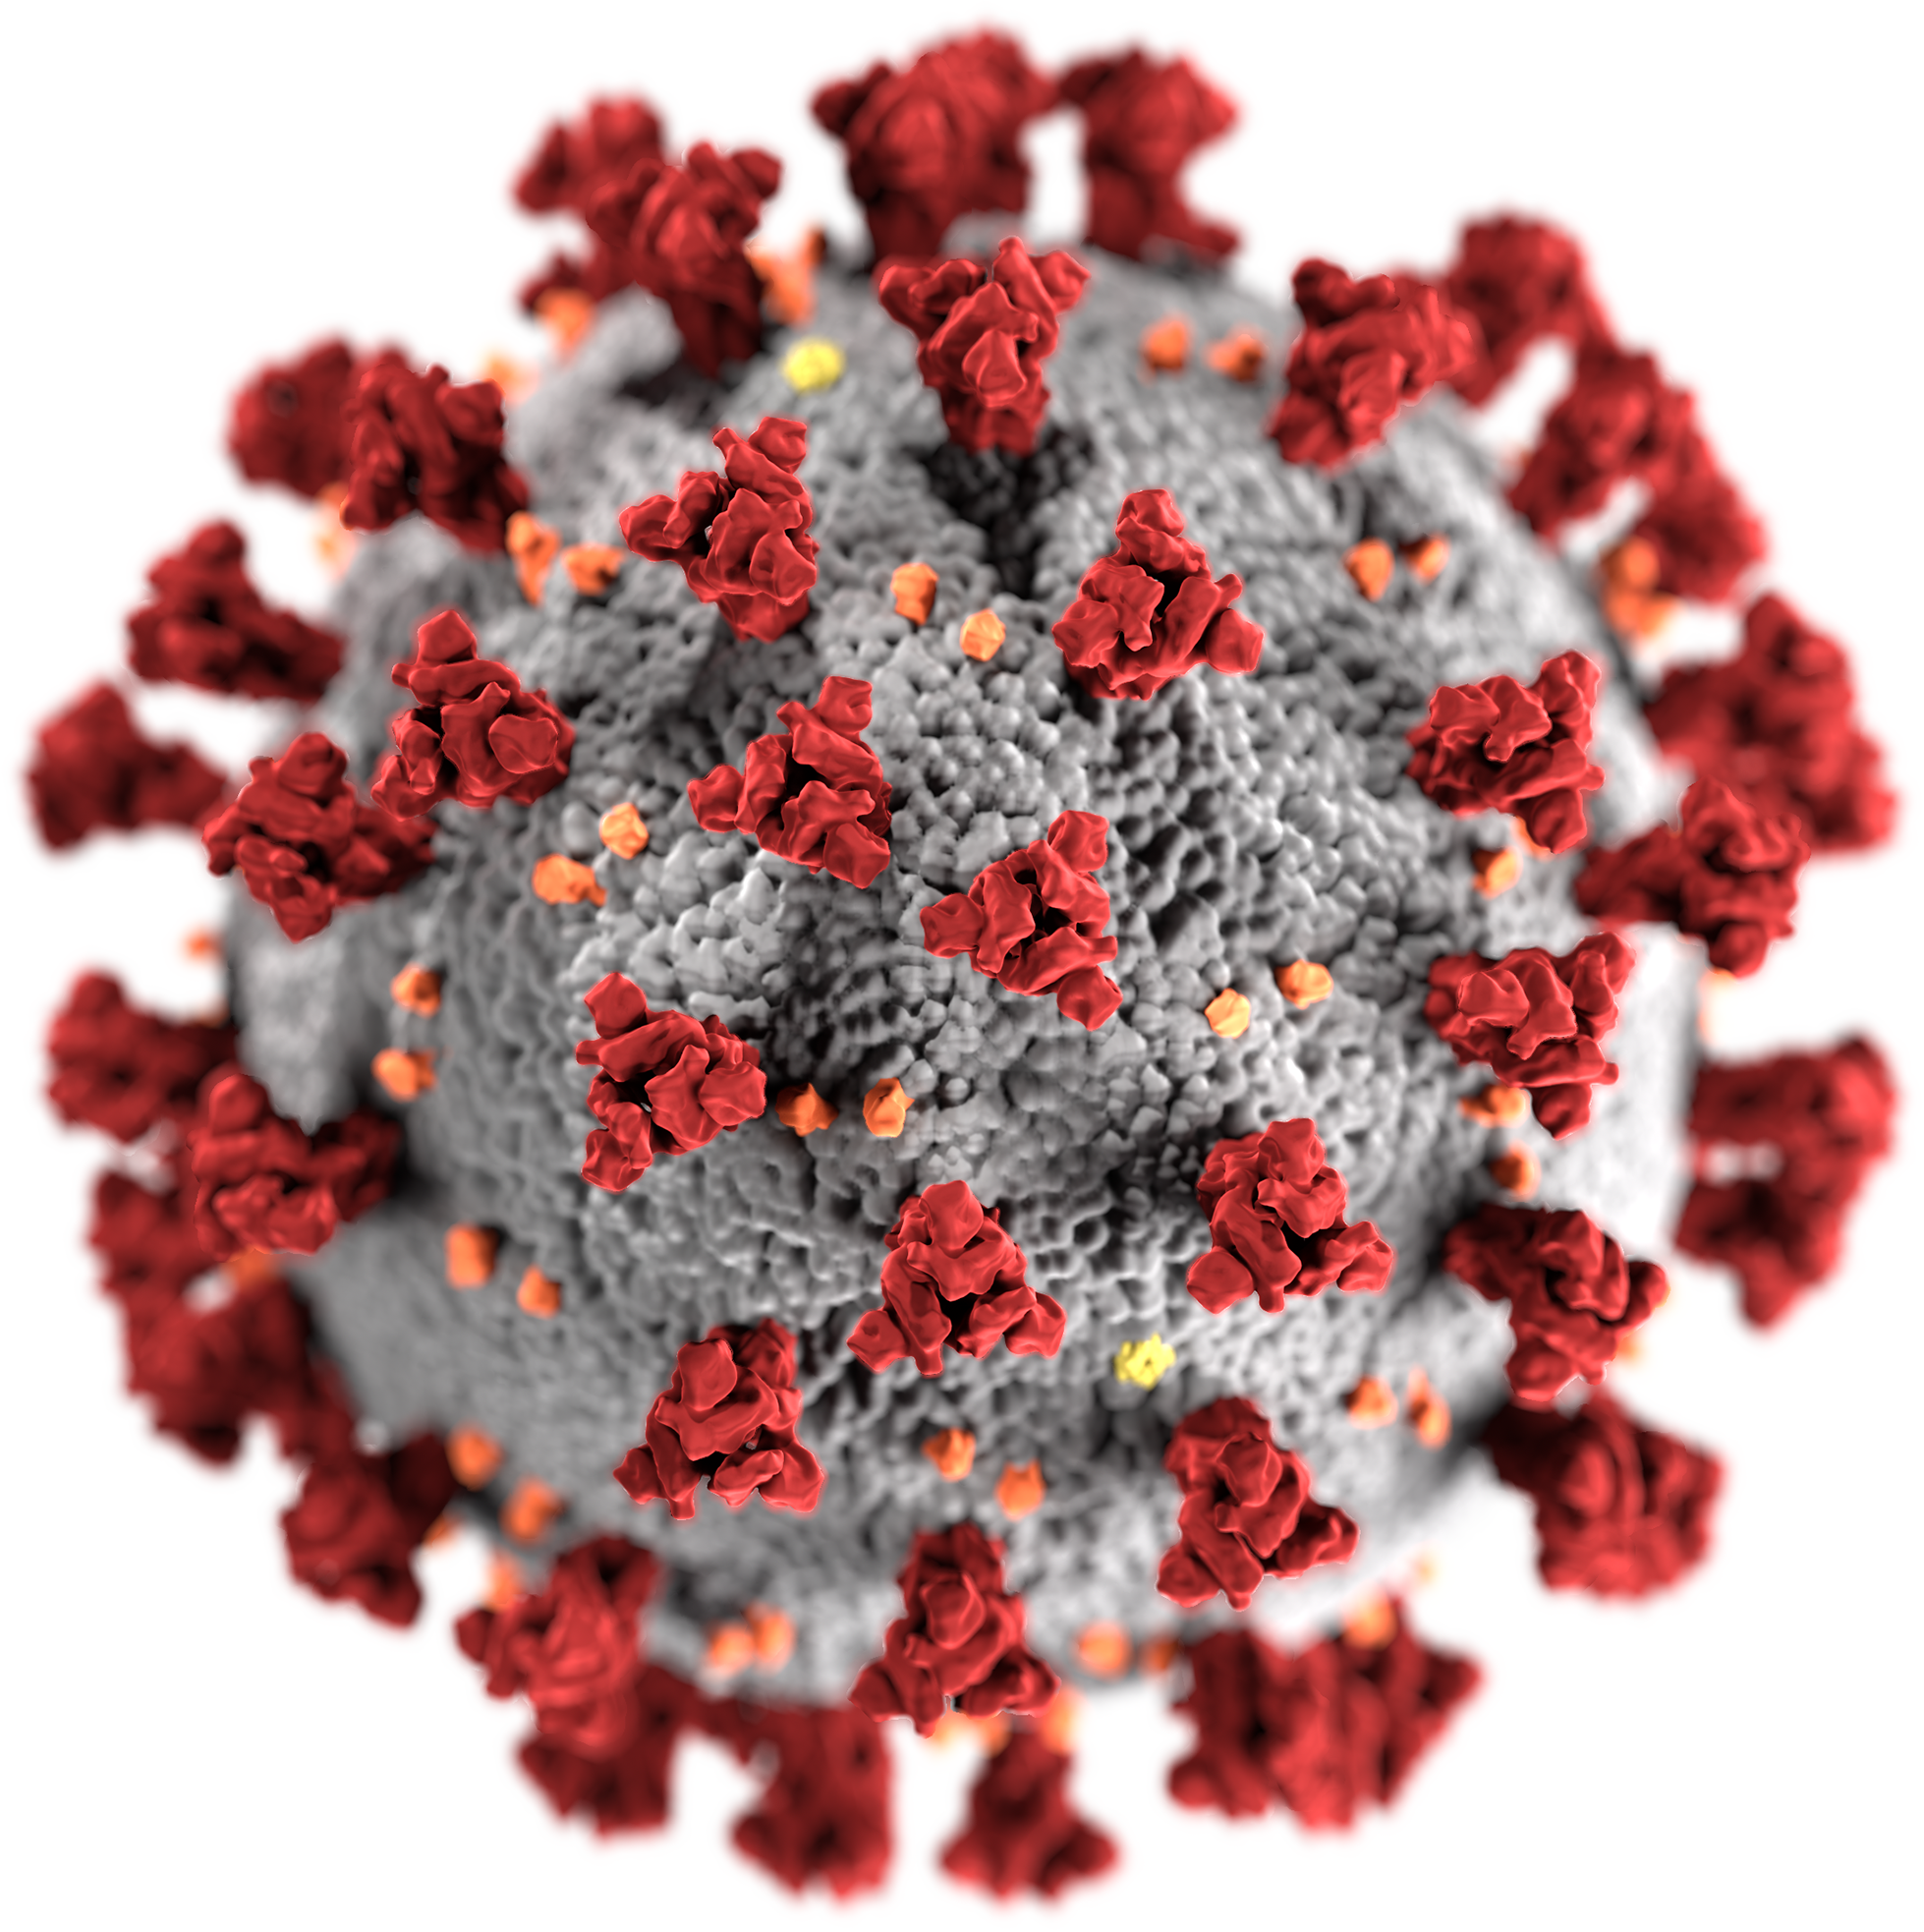
\includegraphics[scale=0.15]{virus1.png}\\[0.5cm]
\end{center}
\end{figure}

\newpage
\begin{abstract}
In this paper we are going to explain the approaches for the mathematical modelling of the spread of infectious diseases such as Coronavirus (COVD-19, SARS-CoV-2). This paper will explain the classic compartmental models in the epidemics literature such as SIR, SIS, SEIR etc. It also explains key concepts such was reproduction number, final size equation, and the key theorems that are implied by these concepts.
\end{abstract}
\renewenvironment{abstract}
{
	\centerline
	{\large \bfseries \scshape Acknowledgement}
	\begin{quote}
	}
	{
	\end{quote}
}
\begin{abstract}
I am writing this acknowledgement on exactly the morning of \textbf{1st of April 2020}. The below is based up to this time.
Any update or new development will be under an \textbf{update} (highlighted in bold) explaining the development of the spread/ with a corresponding date. Consider this section as `diary' preserving the events what might go down in history as modern humanity's most critical events. 

Technology allowed working form home possible, Last time this was done was in University (Possibly the instinct of writing this paper is due to that time in history)

I have started writing this paper on the 18th of March 2020, the date that the UK government enforced `lock-down' - where all the UK work force was compelled to work from home it they could. 

\textbf{17.04.2020: } The lock down has been extended for another 3 weeks.

\end{abstract}
% keywords can be removed
\keywords{First keyword \and Second keyword \and More}


\tableofcontents
\newpage



\section{Introduction}
Coronaviruses are a group of related viruses that cause diseases in mammals and birds. In humans, coronaviruses cause respiratory tract infections that can be mild, such as some cases of the common cold (among other possible causes, predominantly rhinoviruses), and others that can be lethal, such as SARS, MERS, and COVID-19. Symptoms in other species vary: in chickens, they cause an upper respiratory tract disease, while in cows and pigs they cause diarrhea. As of the date of writing this paper, there are yet to be vaccines or antiviral drugs to prevent or treat human coronavirus infections.

Coronavirus has been causing a lot of suffering, public health emergencies, anxiety and economic challenges. It will be of great interest to discuss how mathematical modelling is used to understand and contain the spread of such infectious diseases.

Infectious diseases spread via an infected host to a non-infected host - it very similar to a reproduction process. The agent could be a virus, bacteria, protozoa etc. The role of mathematical modelling is to help estimate the number of infectives over time. Amature modelers tend to use exponential curves to describe the spread of the desease. But this is not how actual mathematical modelling is done in practice. The increase in the number of infectives in the intial stages of the spread looks exponantial, hence the rush to fit an exponential curve. Curve fitting might be good for some applications such as scaremongering\footnote{The spreading of frightening or ominous reports or rumours.}. However the essential dynamics of the essential dynamics of the essential disease process needs to be modelled in order to gain insights into the drivers of the spread and inform the containment strategies.
The questions that one can answer with mathematics could be:
\begin{enumerate}
	\item Will the disease become an epidemic (i.e. large increase in the number of cases with in a short period of time)?
	\item Will the disease become an endemic? (i.e. disappearance or constant prevalence) 
\end{enumerate} 

Once we have reasonable mathematical model of the spread, then we can evaluate the relative effectiveness of various containment strategies. Mathematical models don't require a lot of data, and hence can be quickly put to use. The list of uses of mathematics is boundless, for example at later stages when one has a vaccine, then models can also help determine the optimal vaccination strategy to achieve herd immunity. For example, you are not supposed to capture all the details in a mathematical model - just the essentials. Infectious diseases involve microscopic processes, the little creatures such as virus and bacteria, and their actions and macro variables such as impact on communities. Capturing everything is not going to give you a tractable model, so the priciple of parsimony is the key.

\section{Compartmental Modelling}
\subsection{Introduction}
The classical framework for modelling infectious diseases is the so called compartmental modelling approach. Compartmental models are a technique used to simplify the mathematical modelling of infectious disease. 

Compartmental models may be used to predict properties of how a disease spreads, for example the prevalence (total number of infected) or the duration of an epidemic. Also, the model allows for understanding how different situations may affect the outcome of the epidemic, e.g., what the most efficient technique is for issuing a limited number of vaccines in a given population. 

The models are usually investigated through ordinary differential equations (which are deterministic), but can also be viewed in a stochastic framework, which is more realistic but also more complicated to analyse.


\subsection{Level of Compartments}
The population is divided into compartments, with the assumption that every individual in the same compartment has the same characteristics, below are the compartments:

\begin{description}[leftmargin=!,labelwidth=\widthof{\bfseries Susceptibles}]
	
	\item[Susceptibles] According 
	\item[Infactives] According 
	\item[Removed] According 
	
\end{description}

\section{Compartmental Framework}
\subsection{SIR Framework}

\begin{enumerate}
	\item \textbf{Susceptibles:} In the beginning we have the population of susceptibles (i.e. the individuals that can get infected), which is the first compartment illustrated in figure \ref{fig: full_population}. 
	\item \textbf{Outbreak:} Suddenly there is a virus outbreak\footnote{the reason for the outbreak is beyond the scope of this paper} and one of the individuals gets infected, which is the second compartment illustrated in figure \ref{fig: individual_infection}. 
	\item \textbf{Spread of Infection:} The infected individual then starts to infect other individuals, effectively increasing the number of infective (i.e. expanding the second compartment), this expansion is illustrated in figure \ref{fig: multiple_infections}.
	\item \textbf{Stability:} The spread of infection stabilises or plato's at some point in time, this is illustrated in figure \ref{fig: population_infections}.
	\item \textbf{Removed (Recovery or Death): }Some of the infective recovers or die. This is illustrated in figure \ref{fig: start_removed}.
	\item \textbf{Expansion of Removed: }The recovered compartment grows until covers all the infected compartment, this is both people who have recovered with immunity to the virus, or have died.
	
\end{enumerate}

This is called SIR, so the flow is from susceptibles to infective to removed, this is isllustrated in figure \ref{fig: SIR_flow}. This framework is for diseases where upon recovery, one develops long term immunity to the disease. Generally this is the case for virus based infectious diseases. For diseases caused by bacteria one generally does not develop immunity, so the SIS framework is used for the modelling of these diseases, so the flow is from susceptibles to infective and then back to Susceptibles see figure \ref{fig: SIS_flow}.
Many variations are possible within the compartmental framework. For example, for some diseases, one only gets short term immunity, so there would be an additional flow from R to S, leading to the SIRS framework, this is illustrated in figure \ref{fig: SIRS_flow}. It could be that there is no recovery , and you will then have the SI framework, with just two compartments. This same framework can also be used to model the spread of fake news, so `infected' would then be the people who have the fake news and are spreading it, and the `recovered' are the enlightened. So many variations are possible, but one has to base the choice on how the dynamics of how the infection works.

\begin{figure}
	\begin{center}
		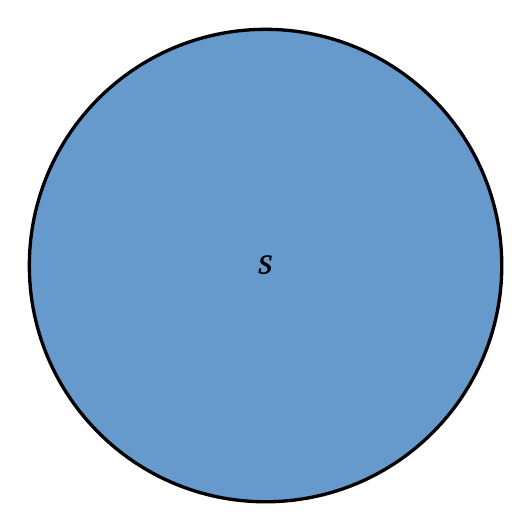
\begin{tikzpicture}
		\node[circle,draw, minimum size=6cm ,fill=bluegray,very thick] (S) at  (0,0){\textbf{\textit{\raisebox{17\height}\Large S}}};
		\end{tikzpicture}
	\end{center}
	\caption{Population of Susceptibles}
	\label{fig: full_population}
\end{figure}

\begin{figure}
	\begin{minipage}{.5\textwidth}
		
		\centering
		\begin{center}
			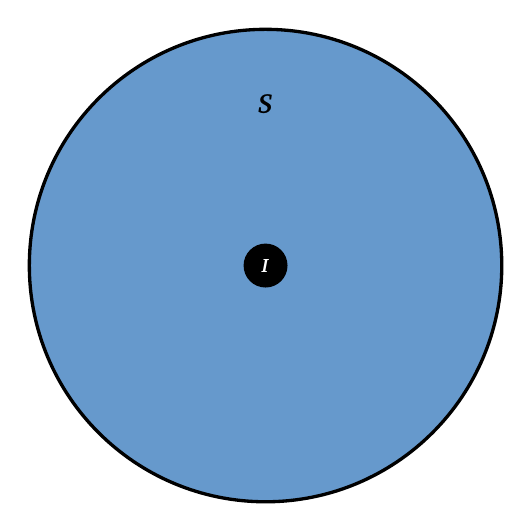
\begin{tikzpicture}
			
			\node[circle,draw, minimum size=6cm ,fill=bluegray,very thick] (S) at  (0,0){\textbf{\textit{\raisebox{17\height}S}}};
			\node[circle,draw, minimum size=0.1cm ,fill=black,very thick] (I) at  (0,0){\textbf{\color{white}\scriptsize \textit{I}}};
			
			\end{tikzpicture}
		\end{center}
		\caption{A Single Infection}
		\label{fig: individual_infection}
	\end{minipage}%
	\begin{minipage}{0.5\textwidth}
	
	\centering
	\begin{center}
		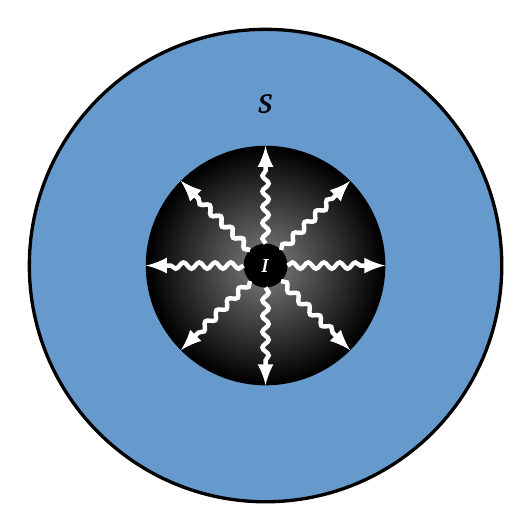
\begin{tikzpicture}
		
		\node[circle,draw, minimum size=6cm ,fill=bluegray,very thick] (A) at  (0,0){\textbf{\textit{\raisebox{17\height}S}}};
		\node[circle,draw, minimum size=3cm ,fill=bluegray,very thick,inner color=gray, outer color=black] (O) at  (0,0){\textbf{\textit{\raisebox{0\height}O}}};
		\node[circle,draw, minimum size=0.1cm ,fill=black,very thick] (B) at  (0,0){\textbf{\color{white}\textit{\scriptsize I}}};
		
		\draw [white!90!white,-latex,ultra thick,decorate,decoration={snake,amplitude=.4mm,segment length=2mm,post length=3mm}] ([xshift=0cm,yshift=0cm]B.north) -- ([xshift=0cm,yshift=0cm]O.north);
		node[midway,below]
		\draw [white!90!white,-latex,ultra thick,decorate,decoration={snake,amplitude=.4mm,segment length=2mm,post length=3mm}] ([xshift=0cm,yshift=0cm]B.north west) -- ([xshift=0cm,yshift=0cm]O.north west);
		node[midway,below]
		
		\draw [white!90!white,-latex,ultra thick,decorate,decoration={snake,amplitude=.4mm,segment length=2mm,post length=3mm}] ([xshift=0cm,yshift=0cm]B.east) -- ([xshift=0cm,yshift=0cm]O.east);
		node[midway,below]
		\draw [white!90!white,-latex,ultra thick,decorate,decoration={snake,amplitude=.4mm,segment length=2mm,post length=3mm}] ([xshift=0cm,yshift=0cm]B.north east) -- ([xshift=0cm,yshift=0cm]O.north east);
		node[midway,below]
		
		\draw [white!90!white,-latex,ultra thick,decorate,decoration={snake,amplitude=.4mm,segment length=2mm,post length=3mm}] ([xshift=0cm,yshift=0cm]B.west) -- ([xshift=0cm,yshift=0cm]O.west);
		node[midway,below]
		\draw [white!90!white,-latex,ultra thick,decorate,decoration={snake,amplitude=.4mm,segment length=2mm,post length=3mm}] ([xshift=0cm,yshift=0cm]B.north west) -- ([xshift=0cm,yshift=0cm]O.north west);
		node[midway,below]
		
		\draw [white!90!white,-latex,ultra thick,decorate,decoration={snake,amplitude=.4mm,segment length=2mm,post length=3mm}] ([xshift=0cm,yshift=0cm]B.south) -- ([xshift=0cm,yshift=0cm]O.south);
		\draw [white!90!white,-latex,ultra thick,decorate,decoration={snake,amplitude=.4mm,segment length=2mm,post length=3mm}] ([xshift=0cm,yshift=0cm]B.south west) -- ([xshift=0cm,yshift=0cm]O.south west);
		node[midway,below]
		\draw [white!90!white,-latex,ultra thick,decorate,decoration={snake,amplitude=.4mm,segment length=2mm,post length=3mm}] ([xshift=0cm,yshift=0cm]B.south east) -- ([xshift=0cm,yshift=0cm]O.south east);
		node[midway,below]
		
		\end{tikzpicture}
		
	\end{center}
	\caption{Infection Spreading}
	\label{fig: multiple_infections}
\end{minipage}%
\end{figure}
\begin{figure}
	\begin{center}
		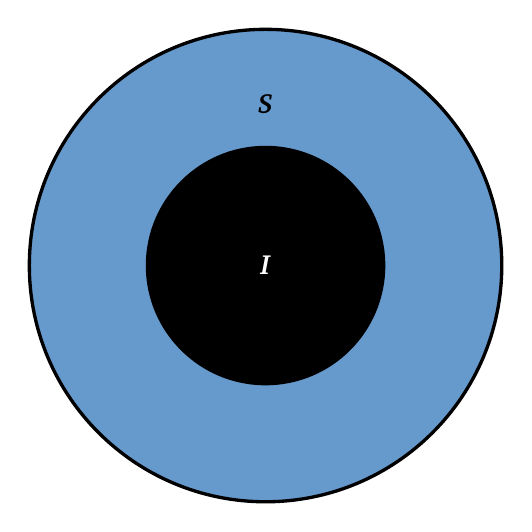
\begin{tikzpicture}
		
		\node[circle,draw, minimum size=6cm ,fill=bluegray,very thick] (A) at  (0,0){\textbf{\textit{\raisebox{17\height}S}}};
		\node[circle,draw, minimum size=3cm ,fill=bluegray,very thick,color=black] (O) at  (0,0){\textbf{\color{white}\textit{\raisebox{0\height}I}}};
		\end{tikzpicture}
	\end{center}
	\caption{Infection Settles}
	\label{fig: population_infections}
\end{figure}

\begin{figure}
	\begin{center}
		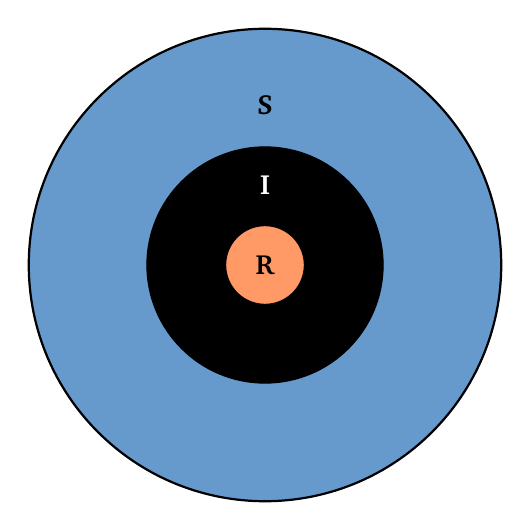
\begin{tikzpicture}
		
		\node[circle,draw, minimum size=6cm ,fill=bluegray,thick] (S) at  (0,0){\textbf{\raisebox{17\height}S}};
		
		\node[circle,draw, minimum size=3cm,fill=black] (I) at  (0,0) { \raisebox{8.5\height}{\color{white}\textbf{I}}};
		
		\node[circle,draw, minimum size=1cm,fill=atomictangerine] (R) at  (0,0){\textbf{\color{black}R}};
		\end{tikzpicture}
	\end{center}
	\caption{Infected start to be `Removed' (i.e. either died or recovered)}
	\label{fig: start_removed}
\end{figure}





% Now we can draw the sets:
\begin{figure}
	\begin{center}
		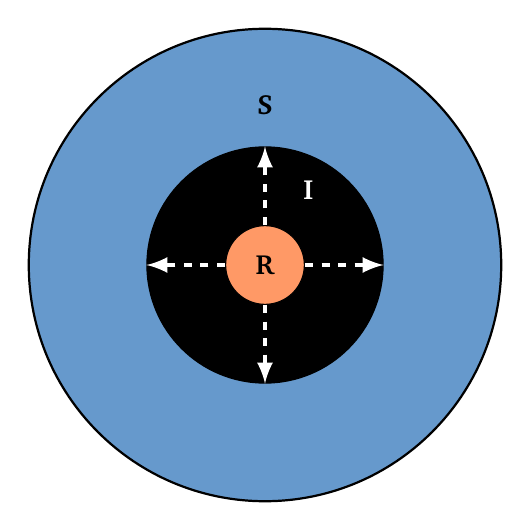
\begin{tikzpicture}
		
		\node[circle,draw, minimum size=6cm ,fill=bluegray,thick] (A) at  (0,0){\textbf{\raisebox{17\height}S}};
		
		\node[circle,draw, minimum size=3cm,fill=black] (B) at  (0,0) {\hspace{1cm} \raisebox{8\height}{\color{white}\textbf{I}}};
		
		\node[circle,draw, minimum size=1cm,fill=atomictangerine] (C) at  (0,0){\textbf{\color{black}R}};
		
		\draw [white!90!white,-latex,ultra thick,dashed] ([xshift=0cm,yshift=0cm]C.north) -- ([xshift=0cm,yshift=0cm]B.north);
		node[midway,below]
		\draw [white!90!white,-latex,ultra thick,dashed] ([xshift=0cm,yshift=0cm]C.east) -- ([xshift=0cm,yshift=0cm]B.east);
		node[midway,below]
		\draw [white!90!white,-latex,ultra thick,dashed] ([xshift=0cm,yshift=0cm]C.west) -- ([xshift=0cm,yshift=0cm]B.west);
		node[midway,below]
		\draw [white!90!white,-latex,ultra thick,dashed] ([xshift=0cm,yshift=0cm]C.south) -- ([xshift=0cm,yshift=0cm]B.south);
		node[midway,below]
		\end{tikzpicture}
	\end{center}
	\caption{`Removed' start to expand within infected}
	\label{fig: expand_removed}
\end{figure}

\begin{figure}
	\begin{center}
		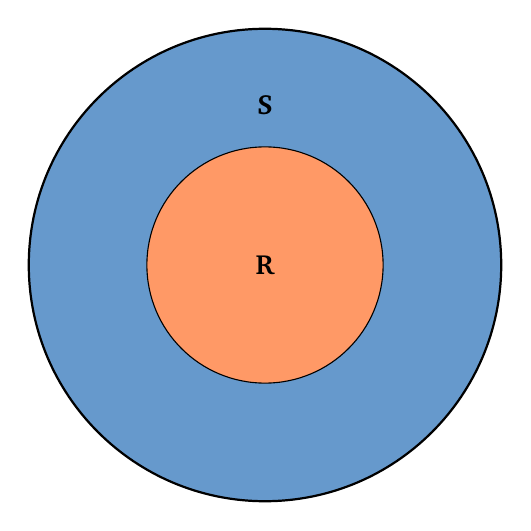
\begin{tikzpicture}
		\node[circle,draw, minimum size=6cm ,fill=bluegray,thick] (S) at  (0,0){\textbf{\raisebox{17\height}S}};
		\node[circle,draw, minimum size=3cm,fill=atomictangerine] (R) at  (0,0) { \raisebox{0\height}{\color{black}\textbf{R}}};
		\end{tikzpicture}
	\end{center}
	
	\caption{All infected are Removed (i.e. either died or recovered)}
	\label{fig: end_removed}
\end{figure}

\subsection{SIR Framework Overview}

Generally, the way infectious diseases spread is through the following:
\begin{enumerate}
	\item \textbf{Contact with Infective: }you get the agent, virus or bacteria, via contact with an infective. 
	\item \textbf{Infectious: }the virus will try to overcome the immune system, and at some point will become Infectious. 
	\item \textbf{Symptoms: }You may or may not have the symptoms yet, but you can spread the disease to others, though the infectivity might be lower than when you start showing symptoms.
	\item \textbf{End of Infectiousness: }As you recover, you will become non-infective.
	\item \textbf{Removed/Recovered: }You recover.
\end{enumerate}
You can add another compartment - `Exposed'. Then the SIR will become SEIR, and SIS will become SEIS etc.

\subsection{Mathematical Modelling of the SIR Framework}

Here we are going to be using deterministic calculus, whcih means that the follows will take the form of differenctial equations. Let's start with the flow from S to I. Individuales flow from S to I when invectives mix with susceptibles, this is similar to a chemical reaction ans the law of mass action applies. Now if there are n susceptibles $\left\lbrace S_{1}, S_{2}, S_{3}... S_{n} \right\rbrace$, and m invectives $\left\lbrace I_{1}, I_{2}, I_{3}... I_{m} \right\rbrace$, then the number of interactions will be of the scale of $S_{t}I_{t}$. These will be vary with time as the individuals flow between the compartments. So the rate of change from S to I, which is the change in the number of susceptibles with respect to time, will be proportional to:

\begin{equation}
	\frac{dS_{t}}{dt}=-\beta S_{t}I_{t}
\end{equation}

Here the $\beta$ represents both the contact rate between the individuals and the probability of transmission of the virus. Similarly, lets represent the rate of flow from I to R, by $\gamma$. The rate of change of of I is captured as the inflow from S minus the outflow to the recovery or dead compartment:

\begin{equation} \label{equ: infected}
\frac{dI_{t}}{dt}=\beta S_{t}I_{t}-\gamma I_{y}
\end{equation}

Finally the rate of change R is just equal to the inflow from the infectives compartment:

\begin{equation}
\frac{dR_{t}}{dt}=\gamma I_{t}
\end{equation}

The sum of these three compartments gives us the total population. The total population:

\begin{equation}
N_{t}=S_{t}+I_{t}+R_{t}
\end{equation}

The total population can change over time due to vital population dynamics, births and deaths, but since we are interested in modelling epidemics, which only lasts for a few months, we can ignore the natural births and deaths, and assume N is constant over time. But it is easy to add the births and deaths if one likes.

These differntial equations are most commonly viewed in terms of population density instead instead of the size of the compartments. For example, you will have division by N on the right hand side of the first differnetial, but it does not mauch difference to the analysis as the total population is constant, so it is just a scaling issue. Other possible variations make the real differnece by enriching the framework. For example, one can make the infectivity a function of time since infection, so now we can get a more realistic model of the actual infection process.

\begin{equation}
\int \beta(\tau)\frac{dS(t-\tau)}{dt}d\tau
\end{equation}


So this equation is essentially taking the infected population, along with the time since they got infected, which is captured by $(t-\tau$. The deivative $\frac{dS_{t}}{dt}$ captures the flows to the infected compartment, and then multiplying by the infectivity $\beta$, which is now a function time since infection. This system is dipicted graphically in figure \ref{fig: SIR_math_flow}

In the simpler version we are considering here, we assumed all currencyle infected people have the same infectivity $\beta$, irspective of time since infection.

For another variation, it is expected that the contact rate, the infectivity rate and the recovery rate could be different for different strata, such as differnrnt age groups. So multiple strata can be introduced into the framework. However solving the system must be known, which may not be as simple, which may lead to resorting to numerical methods.


\subsection{SIS Framework Solution}\label{sec: SIS_solution}
We can solve the SIR system, but let's consider the equivalent SIS first, which is easier because we only have two compartments, the susceptibles and the infected in equation \ref{equ: infected}. The susceptibles compartment equation is modified as the recovered move back into the susceptibles: 

\begin{equation}
\frac{dS_{t}}{dt}=-\beta S_{t}I_{t}-\gamma I_{y}
\end{equation}

Now N, which is the the total population, is fixed:
\begin{equation}
N_{t}=S_{t}+I_{t}
\end{equation}

So we need to solve for either S or I.
 \begin{align*}
\frac{dI_{t}}{dt}=&\beta S_{t}I_{t}-\gamma I_{t} \\
=&\beta (N-I_{t})I_{t}-\gamma I_{t} && \text{\textit{subitute} }(N_{t}-I_{t})\text{ \textit{into} }S_{t}\\
=&\beta NI_{t}-\beta I_{t}^{2}-\gamma I_{t} && \text{\textit{open brackets}}\\
=&(\beta N-\gamma)I_{t}-\beta I_{t}^{2}&& \text{\textit{combine items}}
\end{align*}
 \begin{equation}\label{equ: bernoulli}
\frac{dI_{t}}{dt}=(\beta N-\gamma)I_{t}-\beta I_{t}^{2}
\end{equation}

We just have to solve for I now, and we S plus I equals N, which is a constant, se can determine S easily. This flow is predicted in figure \ref{fig: SIS_math_flow}

Now, the differential equation \ref{equ: bernoulli} is the famous Bernoulli equation. It is not a linear equation but one can easily linearise it by considering the following transformation:

\begin{align}
\label{equ: I} I_{t}=&\frac{1}{y}\\ 
\frac{dI_{t}}{dt}=&\frac{1}{y^{2}}\frac{dy}{dt}
\end{align}

Now let's substitute these into equation \ref{equ: bernoulli}:

 \begin{align}
\frac{1}{y^{2}}\frac{dy}{dt}=&(\beta N-\gamma)\frac{1}{y}-\beta \frac{1}{y^{2}}\\
-\frac{dy}{dt}=&(\beta N-\gamma)y-\beta&& \text{\textit{multiply by }}y^{2}\\
\frac{dy}{dt}+(\beta N-\gamma)y=&\beta&& \text{\textit{rearrange to show in the fimiliar linear differential equation form }}
\end{align}

This equation can be solved via the integrating factor method. The integrating factor for this particular case is defined as the exponential of the integral of the coefficient of y:
\begin{equation}
f=e^{\int_{0}^{t}(\beta N -\gamma)ds}= e^{(\beta N- \gamma)t}
\end{equation}

 \begin{align}
\frac{dy}{dt}+(\beta N-\gamma)y=&\beta&&\\
e^{(\beta N- \gamma)t}\frac{dy}{dt}+e^{(\beta N- \gamma)t}(\beta N-\gamma)y=&e^{(\beta N- \gamma)t}\beta&& \text{\textit{Multiplying by integrating factor}}\\
\frac{d}{dt}(e^{(\beta N- \gamma)t}y)=&e^{(\beta N- \gamma)t}\beta&& \text{\textit{rewrite as product of 2 terms}}\\
e^{(\beta N- \gamma)u}y\Big|_0^t=&\beta \int_{0}^{t}e^{(\beta N- \gamma)u}&& \text{\textit{Integrate from 0 to t}}
\end{align}

The result of the integral on the right hand side will differ depending on whether the term in the exponent is zero. If it is not equal to zero, then we know the integral of the exponential will produce this expression:

 \begin{align}
\beta \int_{0}^{t}e^{(\beta N- \gamma)u}=&\frac{\beta}{\beta N-\gamma}e^{(\beta N- \gamma)u}y\Big|_0^t&& \text{\textit{if} }\beta N-\gamma \neq 0\\
e^{(\beta N- \gamma)t}y_{t}-y_{0}=&\frac{\beta}{\beta N-\gamma}\Big(e^{(\beta N- \gamma)t}-1\Big)&& \text{\textit{Evaluate expression at the upper and lower limits} }
\end{align}

Notice exponential of zero gives 1. On the other hand, if the term in the exponent equals zero $\beta N -\gamma=0$, then the exponential term will become:
\begin{align}
	\frac{dy_{t}}{dt}=&\beta&&\\
	y_{t}-y_{0}=&\beta t&& \text{\textit{Taking intgral from 0 to t}}
\end{align}

Now we introduced this y to linearise the equation. Our object of interest is I, so lets reverse the transformation by recalling equation \ref{equ: I}.

 \begin{align}
e^{(\beta N- \gamma)t}y_{t}-y_{0}=&\frac{\beta}{\beta N-\gamma}\Big(e^{(\beta N- \gamma)t}-1\Big)&&\\
e^{(\beta N- \gamma)t}\frac{1}{I_{t}}-\frac{1}{I_{0}}=&\frac{\beta}{\beta N-\gamma}\Big(e^{(\beta N- \gamma)t}-1\Big)&& \text{\textit{Reverse transformation and substitute } }\frac{1}{y} \text{\textit{ for }} y\\
I_{t}=&\frac{e^{(\beta N- \gamma)t}}{\frac{1}{I_{0}}+\frac{\beta}{\beta N-\gamma}\Big(e^{(\beta N- \gamma)t}-1\Big)}&& \text{\textit{Rearrange to isolate } }I_{t}
\end{align}
We can do the same for the solution where $\beta N -\gamma=0$:

\begin{align}
y_{t}-y_{0}=&\beta t&&\\
\frac{1}{I_{t}}-\frac{1}{I_{0}}=&\beta t&& \text{\textit{Reverse transformation and substitute } }\frac{1}{y} \text{\textit{ for }} y\\
I_{t}=&\frac{1}{\frac{1}{I_{0}}+\beta t}&& \text{\textit{Rearrange to isolate } }I_{t}
\end{align}

So given the parameters, $\beta$ and $\gamma$, and the population size $N$, we have an equation that tells us the number of infectives over time:

\begin{align}
\label{equ: zero_condition}I_{t}=&\frac{1}{\frac{1}{I_{0}}+\beta t}&& \beta N -\gamma=0\\
\label{equ: nonzero_condition}I_{t}=&\frac{e^{(\beta N- \gamma)t}}{\frac{1}{I_{0}}+\frac{\beta}{\beta N-\gamma}\Big(e^{(\beta N- \gamma)t}-1\Big)}&&\beta N -\gamma \neq 0\\
\end{align}

By knowing $I_{t}$ we know $S_{t}$. We can plot $S_{t}$ and $I_{t}$ over time and we will be able to tell the number of cases, whether the disease is going to evovlove into an epidemic. One of the most useful comparisons with more general systems is to plit $I_{t}$ versus $S_{t}$, where it will be a straight downward sloping line, but this diagram is more important when one moves to more complex models.

Now lets see what happens when $t$ goes to infinity. The behaviour of equation \ref{equ: zero_condition} is trival as it goes to zero. As for behaviour of equation \ref{equ: nonzero_condition}, we shift the exponential term down so that it is easy to take the limit:

\begin{equation}
	I_{t}=\frac{1}{\frac{1}{I_{0}}e^{-(\beta N- \gamma)t}+\frac{\beta}{\beta N-\gamma}\Big(1-e^{(\beta N- \gamma)t}\Big)}
\end{equation}
We now have two branches and we also introduce a third and forth branch where the condition is less than zero and larger than zero:
\begin{itemize}
	\item The third condition lets the limit go to zero similar to the first condition
	\item The forth condition lets the exponential term go to zero where we can simplify the equation
\end{itemize}
\begin{align}
\label{equ: zero_conditionv2}I_{t}=&\frac{1}{\frac{1}{I_{0}}+\beta t}&& \beta N -\gamma=0\\
\label{equ: nonzero_conditionv2}\lim_{t \to \inf}I_{t}=&\frac{1}{\frac{1}{I_{0}}e^{-(\beta N- \gamma)t}+\frac{\beta}{\beta N-\gamma}\Big(1-e^{(\beta N- \gamma)t}\Big)}&&\beta N -\gamma \neq 0\\
\lim_{t \to \inf}I_{t}=&0&&\beta N -\gamma < 0\\
\lim_{t \to \inf}I_{t}=&\frac{1}{0+\frac{\beta}{\beta N-\gamma}(1-0)}=\frac{\beta N- \gamma}{\beta}=N-\frac{\gamma}{\beta}&&\beta N -\gamma > 0
\end{align}

Now we can rearrange the inequality to get the memerable result:
\begin{equation}
\beta N -\gamma > 0 \qquad N\frac{\beta}{\gamma}>1
\end{equation}
So we can interperate $\mathscr{R}_{0}=N\frac{\beta}{\gamma}$ as the threashold for whether the disease will become an epidemic. This ratio is called the \textit{reproduction number} or \textit{reproduction ratio} and it is a very important concept in the study of epidemics. This reproduction number ha a very easy interpretation. We know $N\beta$ really means the average number of people infected by one infective per unit of time. Remember the $\gamma$ represents the rate of flow from the infective compartment, so you can see $\frac{1}{\gamma}$ really represents the average time an infective spends in the infectious compartment.

So the reproduction number is the number of secondary infections produced by one primary infective. If one infectious produces more than one infective $\mathscr{R}_{0}>1$, then we have an epidemic, but if it is less than 1 infective $\mathscr{R}_{0}<1$, then we don't have an epidemic.

\subsection{SIR Framework Solution}
Section \ref{sec: SIS_solution} discuses and derived the solution for the SIS framework. This section discuses and derives the slightly complicated SIR framework. 




\bibliographystyle{unsrt} 
%\bibliography{references}  %%% Remove comment to use the external .bib file (using bibtex).
%%% and comment out the ``thebibliography'' section.
%\cite{kour2014real}

%%% Comment out this section when you \bibliography{references} is enabled.
\begin{thebibliography}{1}
	
	\bibitem{kour2014real}
	Ali Al Hayki.
	\newblock Real-time segmentation of on-line handwritten arabic script.
	\newblock In {\em Frontiers in Handwriting Recognition (ICFHR), 2014 14th
		International Conference on}, pages 417--422. IEEE, 2014.
	
\end{thebibliography}
\appendix

% Now we can draw the sets:
\begin{figure}
\begin{center}
	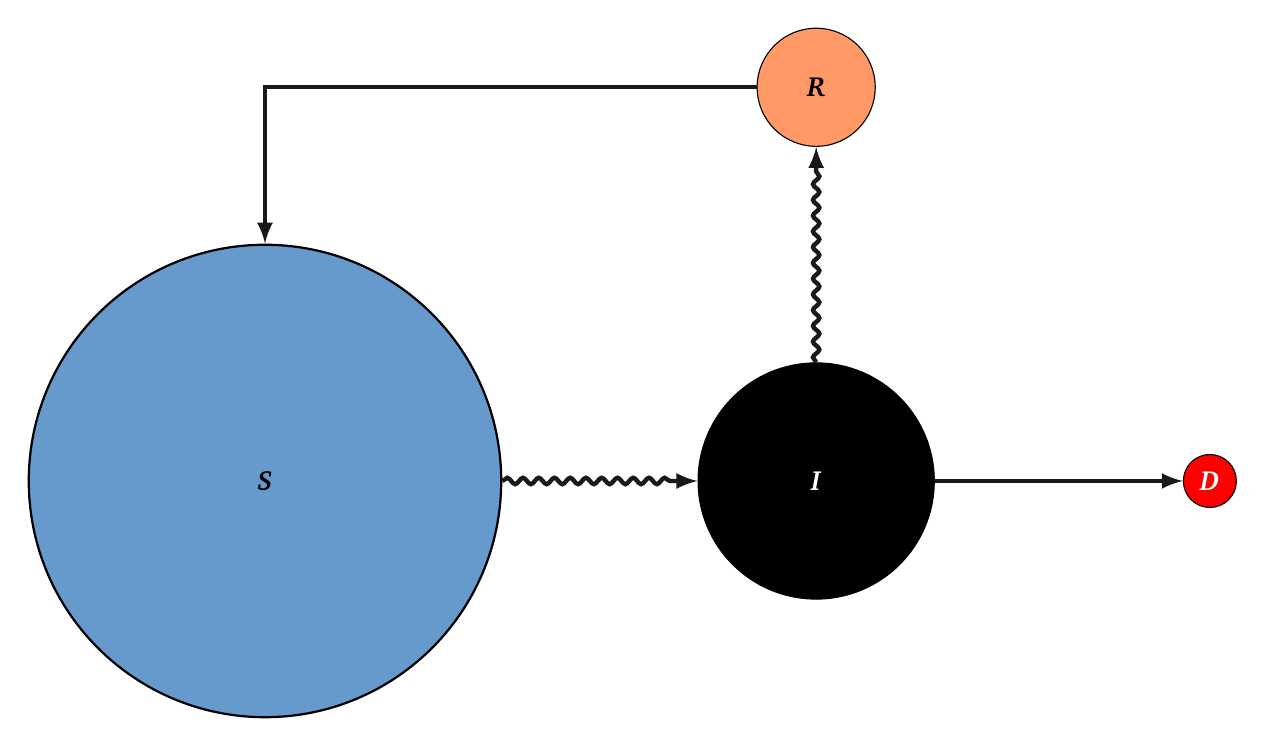
\begin{tikzpicture}

	\node[circle,draw, minimum size=6cm ,fill=bluegray,thick] (A) at  (-12,0){\textbf{\textit{S}}};
	
	\node[circle,draw, minimum size=3cm,fill=black] (B) at  (-5,0) {\textbf{\color{white}\textit{I}}};
	
	\node[circle,draw, minimum size=1.5cm,fill=atomictangerine] (C) at  (-5,5){\textbf{\color{black}\textit{R}}};

	\node[circle,draw, minimum size=0.5cm,fill=red] (D) at  (0,0) {\textbf{\color{white}\textit{D}}};
	
	%\draw[thick] \thirdellipse node[above](C) {\hspace{3.5cm} \raisebox{10\height}{\color{atomictangerine}\textbf{\framebox{A}}}};
	
	
	%\draw [black!90!white,-latex,ultra thick] (A) -- (B);
	\draw[black!90!white,-latex,ultra thick,decorate,decoration={snake,amplitude=.4mm,segment length=2mm,post length=3mm}] (A) -- (B);
	\draw[black!90!white,-latex,ultra thick,decorate,decoration={snake,amplitude=.4mm,segment length=2mm,post length=3mm}] (B) -- (C);
	\draw [black!90!white,-latex,ultra thick] ([xshift=0cm,yshift=0cm]C.west) -| (A);
	node[midway,below]
	\draw [black!90!white,-latex,ultra thick] ([xshift=0cm,yshift=0cm]B.east) -- (D);
	node[midway,below]
	\end{tikzpicture}
\end{center}
		\caption{Infected start to be `Removed' (i.e. either died or recovered)}
\label{fig: SIRS_flow}
\end{figure}

\section{Compartmental Framework}
% Now we can draw the sets:
\begin{figure}
\begin{center}
	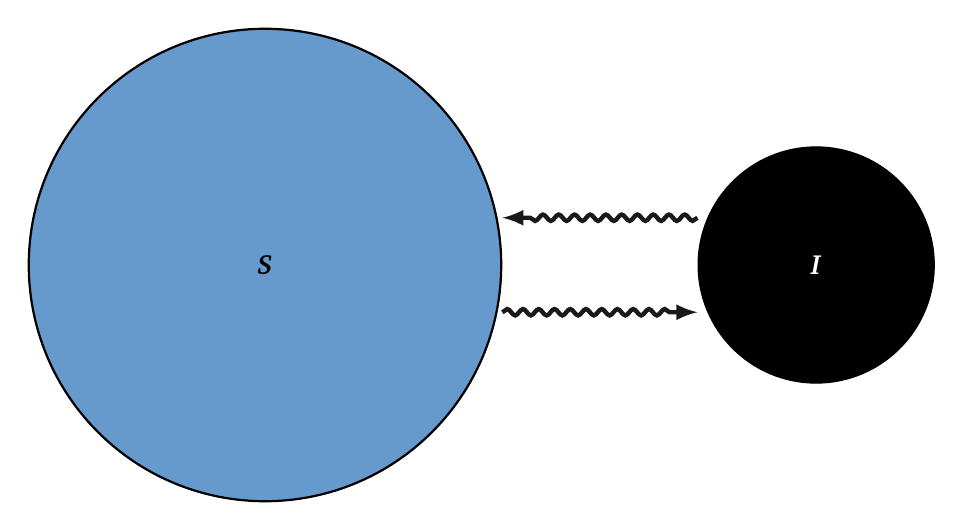
\begin{tikzpicture}
	%\fill[bluegray] \firstellipse ;
	%\fill[black] \secondellipse;
	%\fill[atomictangerine] \thirdellipse ; 
	
	\node[circle,draw, minimum size=6cm ,fill=bluegray,thick] (A) at  (-12,0){\textbf{\textit{S}}};
	
	\node[circle,draw, minimum size=3cm,fill=black] (B) at  (-5,0) {\textbf{\color{white}\textit{I}}};
	
	
	%\draw[thick] \thirdellipse node[above](C) {\hspace{3.5cm} \raisebox{10\height}{\color{atomictangerine}\textbf{\framebox{A}}}};
	
	
	%\draw [black!90!white,-latex,ultra thick] (A) -- (B);
	\draw[black!90!white,-latex,ultra thick,decorate,decoration={snake,amplitude=.4mm,segment length=2mm,post length=3mm}] ($(A.east)-(0,0.6)$) -- ($(B.west)-(0,0.6)$);
	
	\draw[black!90!white,-latex,ultra thick,decorate,decoration={snake,amplitude=.4mm,segment length=2mm,post length=3mm}] ($(B.west)+(0,0.6)$) -- ($(A.east)+(0,0.6)$);
	\end{tikzpicture}
\end{center}
\caption{Infected start to be `Removed' (i.e. either died or recovered)}
\label{fig: SIS_flow}
\end{figure}


\begin{figure}
\begin{center}
	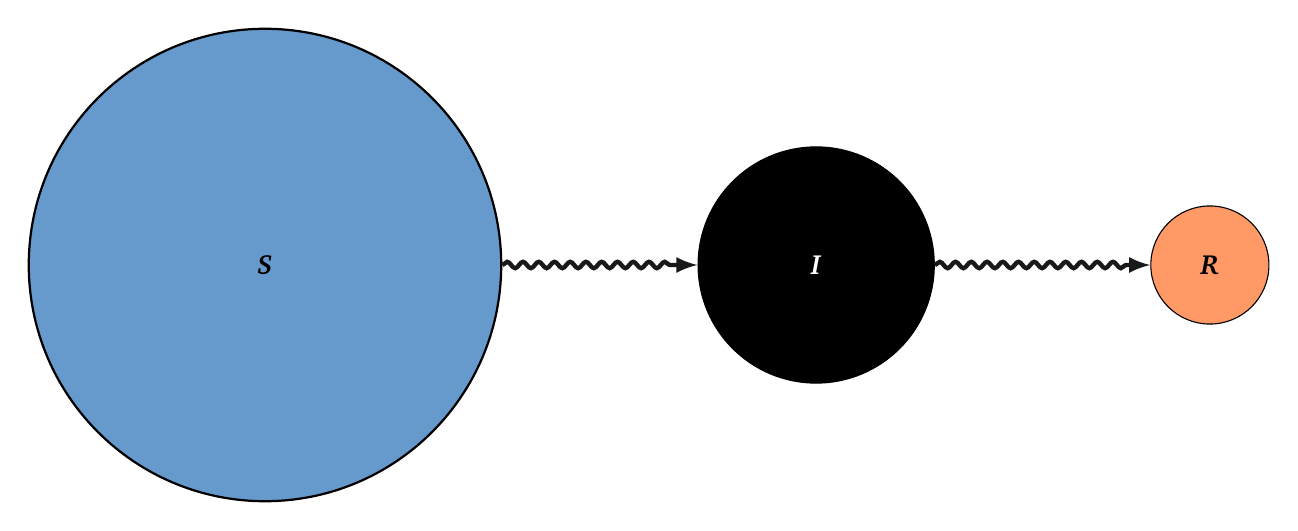
\begin{tikzpicture}
	%\fill[bluegray] \firstellipse ;
	%\fill[black] \secondellipse;
	%\fill[atomictangerine] \thirdellipse ; 
	
	\node[circle,draw, minimum size=6cm ,fill=bluegray,thick] (A) at  (-12,0){\textbf{\textit{S}}};
	
	\node[circle,draw, minimum size=3cm,fill=black] (B) at  (-5,0) {\textbf{\color{white}\textit{I}}};
	
	\node[circle,draw, minimum size=1.5cm,fill=atomictangerine] (C) at  (0,0){\textbf{\color{black}\textit{R}}};
	
	%\draw[thick] \thirdellipse node[above](C) {\hspace{3.5cm} \raisebox{10\height}{\color{atomictangerine}\textbf{\framebox{A}}}};
	
	
	\coordinate (Above A) at ($(A.north)+(0,1.0cm)$);
	\coordinate (Above C) at ($(C.north) + (0,1.0cm)$);
	
	%\draw [black!90!white,-latex,ultra thick] (A) -- (B);
	\draw[black!90!white,-latex,ultra thick,decorate,decoration={snake,amplitude=.4mm,segment length=2mm,post length=3mm}] (A) -- (B);
	\draw[black!90!white,-latex,ultra thick,decorate,decoration={snake,amplitude=.4mm,segment length=2mm,post length=3mm}] (B) -- (C);

	\end{tikzpicture}
\end{center}
\caption{SIR Flow: Susceptibles $\rightarrow$ Infected $\rightarrow$ Removed}
\label{fig: SIR_flow}
\end{figure}


\begin{figure}
 \centering
\begin{minipage}{.5\textwidth}
	\centering
	\begin{equation*}
	N_{t}=S_{t}+I_{t}+R_{t}
	\end{equation*}
	
\begin{center}
	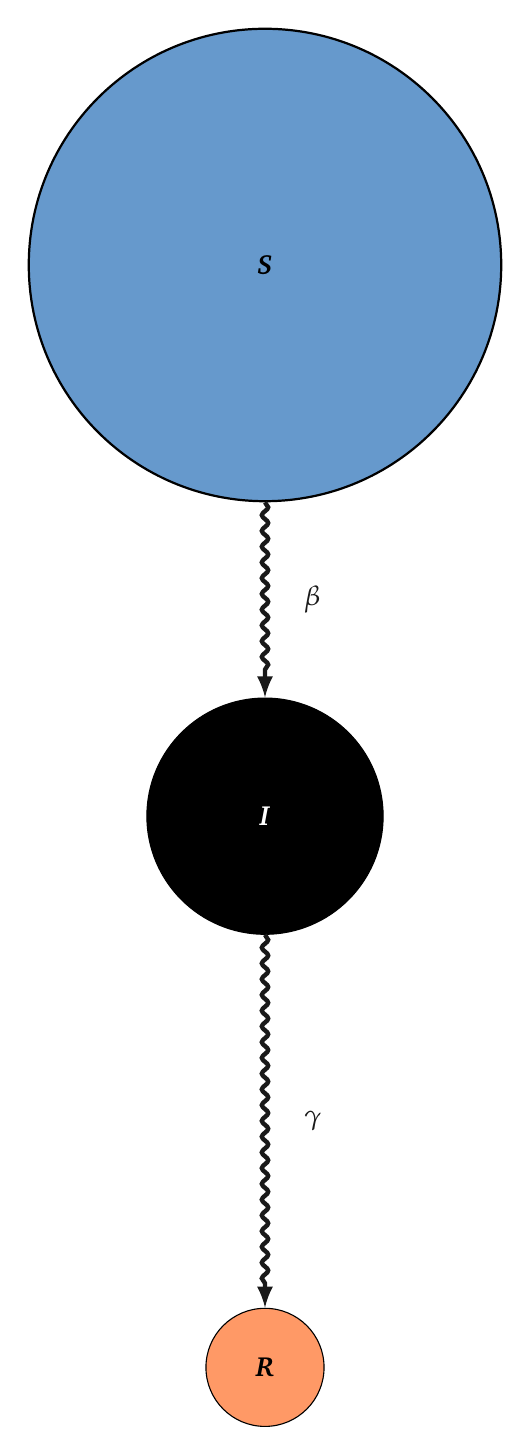
\begin{tikzpicture}
	%\fill[bluegray] \firstellipse ;
	%\fill[black] \secondellipse;
	%\fill[atomictangerine] \thirdellipse ; 
	
	\node[circle,draw, minimum size=6cm ,fill=bluegray,thick] (A) at  (0,10){\textbf{\textit{S}}};
	
	\node[circle,draw, minimum size=3cm,fill=black] (B) at  (0,3) {\textbf{\color{white}\textit{I}}};
	
	\node[circle,draw, minimum size=1.5cm,fill=atomictangerine] (C) at  (0,-4){\textbf{\color{black}\textit{R}}};
		
	
	\coordinate (Above A) at ($(A.north)+(0,1.0cm)$);
	\coordinate (Above C) at ($(C.north) + (0,1.0cm)$);
	
	%\draw [black!90!white,-latex,ultra thick] (A) -- (B);
	\draw[black!90!white,-latex,ultra thick,decorate,decoration={snake,amplitude=.4mm,segment length=2mm,post length=3mm}] (A) -- (B)node[midway,right]{\quad $\beta$};
	
	\draw[black!90!white,-latex,ultra thick,decorate,decoration={snake,amplitude=.4mm,segment length=2mm,post length=3mm}] (B) -- (C)node[midway,right]{\quad $\gamma$};
	
	\end{tikzpicture}
\end{center}
\end{minipage}%
\begin{minipage}{0.5\textwidth}
	\centering
	\begin{tikzpicture}[
	node distance = 6.5cm,
	start chain = A going below,
	dot/.style = {rectangle, draw=white, very thick, fill=gray,
		minimum size=3mm},
	box/.style = {rectangle, text width=62mm,
		inner xsep=7mm, inner ysep=1mm,
		font=\sffamily\small\linespread{0.84}\selectfont,
		on chain},
	]
	\begin{scope}[every node/.append style={box}]
	
	\node {\qquad \qquad \qquad $\frac{dS_{t}}{dt}=-\beta S_{t}I_{t}$ } ;
	
	\node {\qquad \qquad \quad$\frac{dI_{t}}{dt}=\beta S_{t}I_{t}-\gamma I_{t}$ } ;
	
	\node {\qquad \qquad \qquad \qquad$\frac{dR_{t}}{dt}=\gamma I_{t}$};

	\end{scope}
	
	\draw[very thick, black, {Circle[length=4pt)]}-{Circle[length=4pt]},
	shorten <=-4cm, shorten >=-1cm]           % <--- here is adjusted additional arrow's 
	(A-1.north west) -- (A-3.south west);
	%($(A.east)-(0,0.6)$) -- ($(B.west)-(0,0.6)$)
	
	\draw[very thick, black,]($(A-1.north west)-(0,0)$) -- ($(A-2.south west)-(0,0)$)node[yshift=20ex,right]{\hspace{0.1em} $\beta I_{t}$\quad $\int\beta(\tau)\frac{dS(t-\tau)}{dt}d\tau$};

	\draw[thick, black,dashed,-latex,shorten >=0.5cm,shorten <=0.5cm](A-1.south) -- (A-2.north)node[midway,right]{};
	
	\draw[thick, black,dashed,-latex,shorten >=0.5cm,shorten <=0.5cm](A-2.south) -- (A-3.north)node[midway,right]{};
	
	\draw[very thick, black,](A-2.north west) -- (A-3.south west)node[midway,right]{};

	%\foreach \i [ count=\j] in {2013,2010,2006,}
	%\node[dot,label=left:\i] at (A-\j.west) {};
	\node[dot,label=left:S] at (A-1.west) {};
	\node[dot,label=left:I] at (A-2.west) {};
	\node[dot,label=left:R] at (A-3.west) {};
	\end{tikzpicture}
\end{minipage}
\caption{SIR Mathematical Flow: Susceptibles $\rightarrow$ Infected $\rightarrow$ Removed}
\label{fig: SIR_math_flow}
\end{figure}


\begin{figure}
\centering
\begin{minipage}{.5\textwidth}
	\centering
	\begin{equation*}
	N_{t}=S_{t}+I_{t}+R_{t}
	\end{equation*}
	
	\begin{center}
		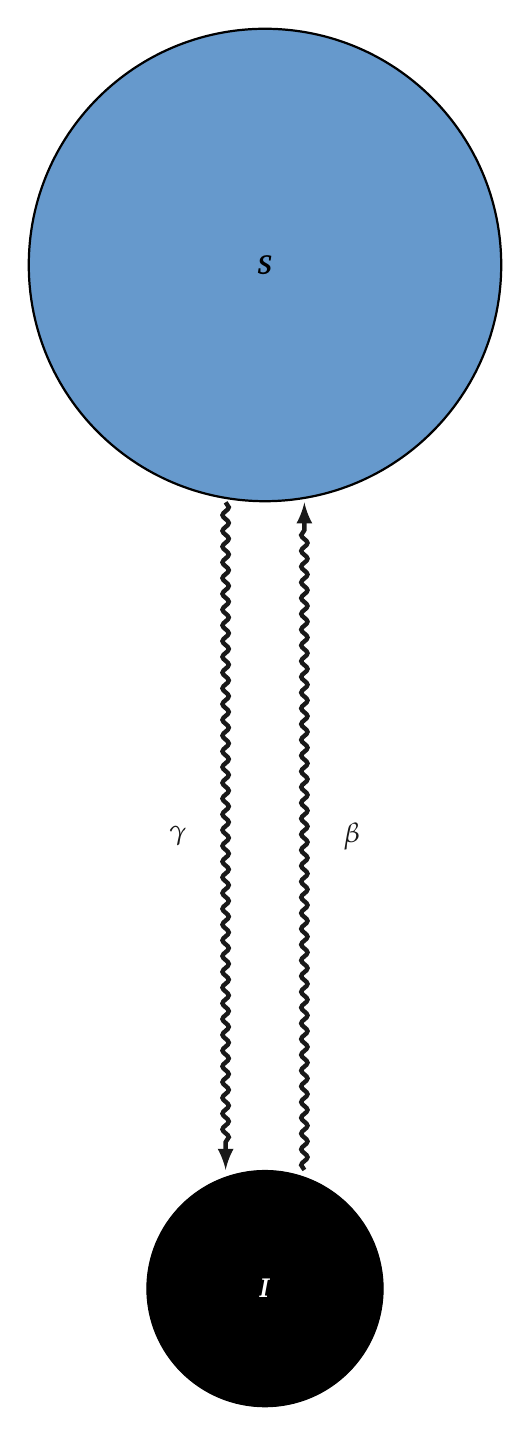
\begin{tikzpicture}
		
		\node[circle,draw, minimum size=6cm ,fill=bluegray,thick] (A) at  (0,15){\textbf{\textit{S}}};
		
		\node[circle,draw, minimum size=3cm,fill=black] (B) at  (0,2) {\textbf{\color{white}\textit{I}}};
		
		\coordinate (Above A) at ($(A.north)+(0,1.0cm)$);
		
		%\draw [black!90!white,-latex,ultra thick] (A) -- (B);
		
		%($(B.west)+(0,0.6)$) -- ($(A.east)+(0,0.6)$);
		\draw[black!90!white,-latex,ultra thick,decorate,decoration={snake,amplitude=.4mm,segment length=2mm,post length=3mm}]($(A.south)-(0.5,0)$) -- ($(B.north)-(0.5,0)$)node[midway,left]{$\gamma \quad$ };

		\draw[black!90!white,-latex,ultra thick,decorate,decoration={snake,amplitude=.4mm,segment length=2mm,post length=3mm}]($(B.north)+(0.5,0)$) -- ($(A.south)+(0.5,0)$)node[midway,right]{\quad $\beta$};
		
		\end{tikzpicture}
	\end{center}
\end{minipage}%
\begin{minipage}{0.5\textwidth}
	\centering
	\begin{tikzpicture}[
	node distance = 11.3cm,
	start chain = A going below,
	dot/.style = {rectangle, draw=white, very thick, fill=gray,
		minimum size=3mm},
	box/.style = {rectangle, text width=62mm,
		inner xsep=7mm, inner ysep=1mm,
		font=\sffamily\small\linespread{0.84}\selectfont,
		on chain},
	]
	\begin{scope}[every node/.append style={box}]
	\node {\qquad \quad $\frac{dS_{t}}{dt}=-\beta S_{t}I_{t}+\gamma I_{t}$} ;
	\node { \begin{align*}
		\frac{dI_{t}}{dt}=&\beta S_{t}I_{t}-\gamma I_{t}\\
		=&\beta (N-I_{t})I_{t}-\gamma I_{t}\\
		=&\beta NI_{t}-\beta I_{t}^{2}-\gamma I_{t}\\
		=&(\beta N-\gamma)I_{t}-\beta I_{t}^{2}
		\end{align*}} ;
	
	\end{scope}
	
	\draw[very thick, black, {Circle[length=4pt)]}-{Circle[length=4pt]},
	shorten <=-4cm, shorten >=-1cm]           % <--- here is adjusted additional arrow's 
	(A-1.north west) -- (A-3.south west);
	%($(A.east)-(0,0.6)$) -- ($(B.west)-(0,0.6)$)
	
	\draw[very thick, black,]($(A-1.north west)-(0,0)$) -- ($(A-2.south west)-(0,0)$)node[yshift=20ex,right]{};
	
	
	%\foreach \i [ count=\j] in {2013,2010,2006,}
	%\node[dot,label=left:\i] at (A-\j.west) {};
	\node[dot,label=left:S] at (A-1.west) {};
	\node[dot,label=left:I] at (A-2.west) {};
	\end{tikzpicture}
\end{minipage}
\caption{SIS Mathematical Flow: Susceptibles $\rightarrow$ Infected $\rightarrow$ Removed}
\label{fig: SIS_math_flow}
\end{figure}

\begin{figure}
	
\centering
\begin{minipage}{.5\textwidth}
	\centering
	
	\begin{center}
		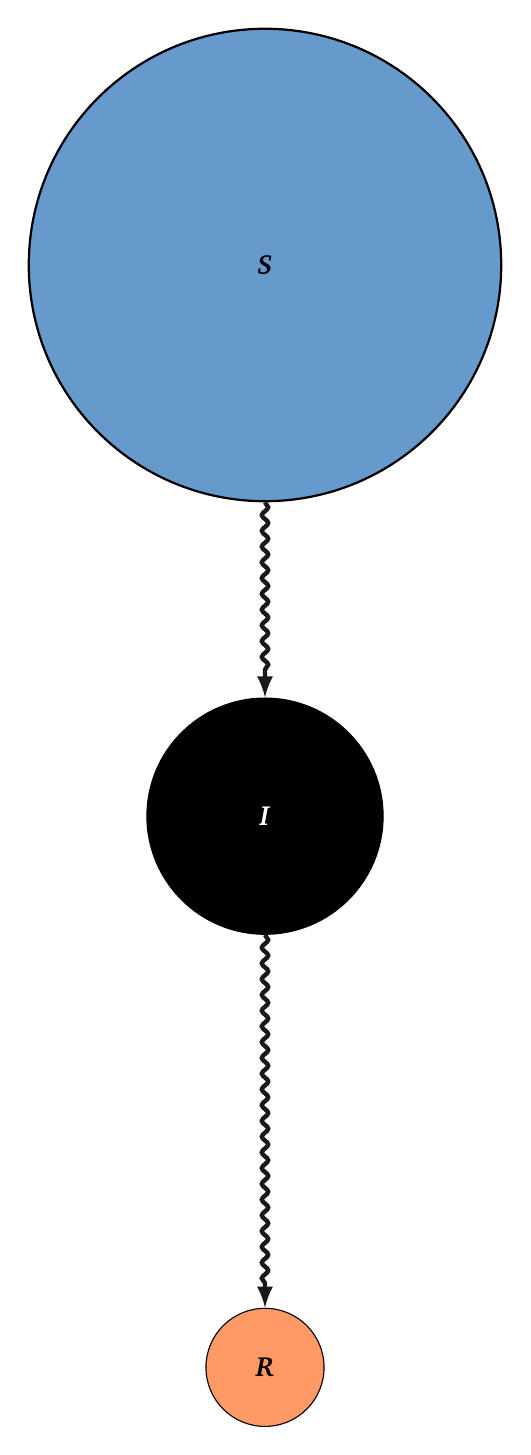
\begin{tikzpicture}
		%\fill[bluegray] \firstellipse ;
		%\fill[black] \secondellipse;
		%\fill[atomictangerine] \thirdellipse ; 
		
		\node[circle,draw, minimum size=6cm ,fill=bluegray,thick] (A) at  (0,10){\textbf{\textit{S}}};
		
		\node[circle,draw, minimum size=3cm,fill=black] (B) at  (0,3) {\textbf{\color{white}\textit{I}}};
		
		\node[circle,draw, minimum size=1.5cm,fill=atomictangerine] (C) at  (0,-4){\textbf{\color{black}\textit{R}}};
		
		
		\coordinate (Above A) at ($(A.north)+(0,1.0cm)$);
		\coordinate (Above C) at ($(C.north) + (0,1.0cm)$);
		
		%\draw [black!90!white,-latex,ultra thick] (A) -- (B);
		\draw[black!90!white,-latex,ultra thick,decorate,decoration={snake,amplitude=.4mm,segment length=2mm,post length=3mm}] (A) -- (B)node[midway,right]{};
		\draw[black!90!white,-latex,ultra thick,decorate,decoration={snake,amplitude=.4mm,segment length=2mm,post length=3mm}] (B) -- (C);
		
		\end{tikzpicture}
	\end{center}
\end{minipage}%
\begin{minipage}{0.5\textwidth}
	\centering
	\begin{tikzpicture}[
	node distance = 6.5cm,
	start chain = A going below,
	dot/.style = {rectangle, draw=white, very thick, fill=gray,
		minimum size=3mm},
	box/.style = {rectangle, text width=62mm,
		inner xsep=7mm, inner ysep=1mm,
		font=\sffamily\small\linespread{0.84}\selectfont,
		on chain},
	]
	\begin{scope}[every node/.append style={box}]
	
	\node {\qquad \qquad \quad Contact with Infective } ;
	
	\node {\qquad \qquad \qquad \quad Symptoms } ;
	
	\node {\qquad \qquad \quad Removed / Recovered};
	
	\end{scope}
	
	\draw[very thick, black, {Circle[length=4pt)]}-{Circle[length=4pt]},
	shorten <=-4cm, shorten >=-1cm]           % <--- here is adjusted additional arrow's 
	(A-1.north west) -- (A-3.south west);
	%($(A.east)-(0,0.6)$) -- ($(B.west)-(0,0.6)$)
	
	\draw[very thick, black,]($(A-1.north west)-(0,0)$) -- ($(A-2.south west)-(0,0)$)node[yshift=20ex,right]{\hspace{0.25em} \color{red}\textit{Infectious}};
	
	\draw[thick, black,dashed,-latex,shorten >=0.5cm,shorten <=0.5cm](A-1.south) -- (A-2.north)node[midway,right]{};
	
	\draw[thick, black,dashed,-latex,shorten >=0.5cm,shorten <=0.5cm](A-2.south) -- (A-3.north)node[midway,right]{};
	
	\draw[very thick, black,](A-2.north west) -- (A-3.south west)node[yshift=20ex,right]{\hspace{0.25em} \color{red}\textit{End of Infectiousness}};
	
	%\foreach \i [ count=\j] in {2013,2010,2006,}
	%\node[dot,label=left:\i] at (A-\j.west) {};
	\node[dot,label=left:\textit{S}] at (A-1.west) {};
	\node[dot,label=left:\textit{I}] at (A-2.west) {};
	\node[dot,label=left:\textit{R}] at (A-3.west) {};
	\end{tikzpicture}
\end{minipage}
\caption{SIR Descriptive Flow: Susceptibles $\rightarrow$ Infected $\rightarrow$ Removed}
\label{fig: SIS_des_flow}
\end{figure}






\end{document}
